\section{Controller tuning}
\subsection{}

\begin{frame}
\frametitleTC{Outline}
\framesubtitleTC{}
\myPause
 \begin{itemize}[<+-| alert@+>]
 \item We stick to the PI case, adding D afterwards is easy.
 \item We first address the pure DT (not sampled-signals) case: % with two frequently encountered structures for $P(z).
 \item the purpose here is to strengthen the comprehension already achieved, while looking also at the behaviour of $u$ and not only $y$.
 \item Then we move to the sampled-signals case:
 \item the purpose is to understand how ``$T_s$-independent'' parameters\\
       can be defined.
 \end{itemize}
\end{frame}

\begin{frame}
\frametitleTC{Pure DT case}
\framesubtitleTC{Dominantly first-order asymptotically stable process}
\myPause
 \begin{itemize}[<+-| alert@+>]
 \item We already saw this:
       \begin{displaymath}
        \begin{array}{l}
          P(z)              = \frac{\mu}{z-p} \\
          G_{yw}^{\circ}(z) = \frac{1-\alpha}{z-\alpha}
          \text{ or }
          G_{yd}^{\circ}(z) = \frac{z-1}{z-\alpha}       
        \end{array}
        \quad \Rightarrow \quad
        C_{PI}(z) = K\,\frac{z-\zeta}{z-1}, \quad
        K         = \frac{1-\alpha}{\mu}, \;
        \zeta     = p.
       \end{displaymath}
 \item The tuning above fulfils our desires on $y$; what about $u$?
 \item We have
       \begin{displaymath}
        \begin{array}{rclclcl}
         G_{uw}(z) &=& \frac{C(z)}{1+L(z)}
                   &=& \frac{\frac{1-\alpha}{\mu}\frac{z-p}{z-1}}{1+\frac{1-\alpha}{z-1}}
                   &=& \frac{1-\alpha}{\mu}\frac{z-p}{z-\alpha}, \\
         G_{ud}(z) &=& \frac{-C(z)}{1+L(z)}
                   &=& -G_{uw}(z)
                   &=& \frac{\alpha-1}{\mu}\frac{z-p}{z-\alpha}. \\
        \end{array}
       \end{displaymath}
 \end{itemize}
\end{frame}

\begin{frame}
\frametitleTC{Pure DT case}
\framesubtitleTC{Dominantly first-order asymptotically stable process}
\myPause
 \begin{itemize}[<+-| alert@+>]
 \item Turning $G_{uw}(z)$ to time domain we get
       \begin{displaymath}
         \begin{array}{rcl}
          \frac{u(k)}{w(k)}  &=& \frac{1-\alpha}{\mu}\frac{z-p}{z-\alpha} \\  
          (z-\alpha) u(k)    &=& \frac{1-\alpha}{\mu}(z-p) w(k) \\
          u(k+1)-\alpha u(k) &=& \frac{1-\alpha}{\mu} \left( w(k+1)-pw(k) \right)
         \end{array}
       \end{displaymath}
 \item and finally, rearranging and scaling the time index,
       \begin{displaymath}
        u(k) = \alpha u(k-1)+\frac{1-\alpha}{\mu} \left( w(k)-pw(k-1) \right).
       \end{displaymath}
 \end{itemize}
\end{frame}

\begin{frame}
\frametitleTC{Pure DT case}
\framesubtitleTC{Dominantly first-order asymptotically stable process}
\myPause
 \begin{itemize}[<+-| alert@+>]
 \item We now analyse the response of $u$ to a step on $w$ (the $d$ case differs only\\
       by the sign):
       {\small
       \begin{displaymath}
         \begin{array}{rclclcl}
          u(0) &=& \alpha u(-1)   + \frac{1-\alpha}{\mu} \left( w(0) - p       w(-1) \right)
               &=& \alpha \cdot 0 + \frac{1-\alpha}{\mu} \left( 1    - p \cdot 0     \right)
               &=& \frac{1-\alpha}{\mu} \\
          u(1) &=& \alpha u(0)    + \frac{1-\alpha}{\mu} \left( w(1) - p       w(0)  \right)
               &=& \alpha \cdot \frac{1-\alpha}{\mu} + \frac{1-\alpha}{\mu} \left( 1-p\right)
               &=& \frac{1-\alpha}{\mu} (1+\alpha-p) \\
          \cdots\\
         \end{array}
       \end{displaymath}
       }
 \item For $k\rightarrow\infty$, then,
       \begin{displaymath}
        u(\infty) = G_{uw}(1) \cdot 1
                  =  \frac{\cancel{1-\alpha}}{\mu}\frac{1-p}{\cancel{1-\alpha}}
                  = \frac{1-p}{\mu}.
       \end{displaymath}
 \end{itemize}
\end{frame}

\begin{frame}
\frametitleTC{Pure DT case}
\framesubtitleTC{Dominantly first-order asymptotically stable process}
\myPause
 \begin{itemize}[<+-| alert@+>]
 \item The response of $u$ to a $w$ (or $d$ if not for the sign) step, thus, can have an initial\\
       overshoot or not:
       \begin{center}
        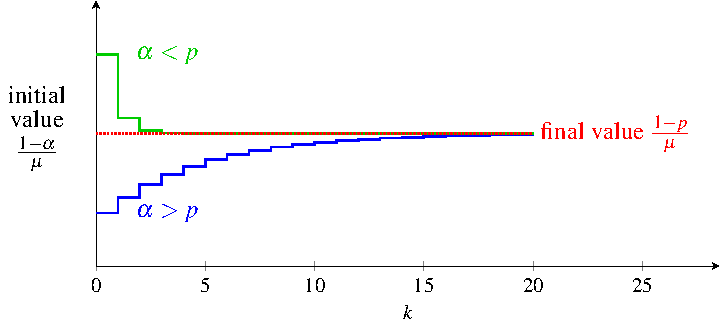
\includegraphics[width=0.55\columnwidth]{./Unit-06/img/ControlStepResponses-1.pdf}
       \end{center}
 \item The analysis we carried out, provides \TC{dynamic} actuator sizing clues:
       \begin{itemize}[<+-| alert@+>]
       \item to sustain \TC{steady state}, must be capable of exerting $u_{max}=\frac{1-p}{\mu} w_{max}$;
       \item if control has to \TC{accelerate} the system ($\alpha<p$) must transiently exert\\
             the \TC{larger} value $u_{max}=\frac{1-\alpha}{\mu} w_{max}$.
       \end{itemize}
 \item Analogous considerations based on the maximum amplitude of $d$,\\
       and the required speed for its rejection, are left as a simple exercise.
 \end{itemize}
\end{frame}

\begin{frame}
\frametitleTC{Pure DT case}
\framesubtitleTC{One-step delayed integrator}
\myPause
 \begin{itemize}[<+-| alert@+>]
 \item A process structure quite frequently encountered in computer-related controls,\\
       is the \TC{one-step delayed integrator}
       \begin{displaymath}
        P(z) = \frac{\mu}{z-1}.
       \end{displaymath}
 \item The name is motivated by the time-domain formulation
       \begin{displaymath}
        y(k) = y(k-1) + \mu u(k-1),
       \end{displaymath}
       showing that at step $k$, $y$ is the sum (DT integral) of $\mu u$ up to the\\
       previous step $k-1$.
 \end{itemize}
\end{frame}

\begin{frame}
\frametitleTC{Pure DT case}
\framesubtitleTC{One-step delayed integrator}
\myPause
 \begin{itemize}[<+-| alert@+>]
 \item If we apply the same policy we used for the stable asymptotically case just setting $p=1$, we get
       \begin{displaymath}
        \begin{array}{l}
          P(z)              = \frac{\mu}{z-1} \\
          G_{yw}^{\circ}(z) = \frac{1-\alpha}{z-\alpha}
          \text{ or }
          G_{yd}^{\circ}(z) = \frac{z-1}{z-\alpha}       
        \end{array}
        \quad \Rightarrow \quad
        C_{PI}(z)  = K\,\frac{z-\zeta}{z-1}, \quad
        K          = \frac{1-\alpha}{\mu}, \;
        \red{\zeta = 1}.
       \end{displaymath}
 \item But we are NOT realising a controller with \red{a zero/pole cancellation on the circle},\\
       as this would create a non asymptotically stable hidden part in the closed-loop\\
       system.
\item Hence we only use the P controller
       \begin{displaymath}
        C(z) = \frac{1-\alpha}{\mu}.
       \end{displaymath}
      and we are back to the case we already treated.
 \end{itemize}
\end{frame}

\begin{frame}[fragile]
\frametitleTC{Sampled-signal case}
\framesubtitleTC{Dominantly first-order asymptotically stable process}
\myPause
 \begin{itemize}[<+-| alert@+>]
 \item Just a bit of CT: if we take the first-order LTI system
       \begin{displaymath}
        \dot{y}(t) = ay(t)+bu(t)
       \end{displaymath}
 \item and set $y(0)=0$, $u(t)=1$ for $t \geq 0$ to compute its unit step response, we get
       \begin{displaymath}
        y(t) = \frac{b}{a} \left( e^{at}-1 \right)
       \end{displaymath}
 \item Check (wxMaxima):
       \begin{verbatim}
  y: b/a*(exp(a*t)-1);
  u: 1;
  ratsimp(diff(y,t)-(a*y+b*u)); /* -> zero, OK */
  subst(t=0,y);                 /* -> zero, OK */
       \end{verbatim}
 \end{itemize}
\end{frame}

\begin{frame}
\frametitleTC{Sampled-signal case}
\framesubtitleTC{Dominantly first-order asymptotically stable process}
\myPause
 \begin{itemize}[<+-| alert@+>]
 \item Incidentally, the response converges for $a<0$ (system asymptotically stable),\\
       is constant for $a=0$ (simply stable) and diverges for $a>0$ (unstable).
 \item Generalising to orders above one, there is a stability theorem for CT systems\\
       identical to the one we know for DT ones, if not for replacing ``magnitude\\
       of eigenvalue of $A$ $\lesseqgtr$ 1'' with ``real part of eigenvalue of $A$ $\lesseqgtr$ 0''.\\
 \item Enough for us here.
 \end{itemize}
\end{frame}

\begin{frame}
\frametitleTC{Sampled-signal case}
\framesubtitleTC{Dominantly first-order asymptotically stable process}
\myPause
 \begin{itemize}[<+-| alert@+>]
 \item If we re-write the CT system above with differently named parameters, i.e.,
       \begin{displaymath}
        \dot{y}(t) = -\frac{1}{T}y(t) + \frac{\mu}{T} u(t)
       \end{displaymath}
 \item[] where asymptotic stability means $T>0$, the unit step response takes the form
       \begin{displaymath}
        y(t) = \mu \left( 1-e^{-t/T} \right).
       \end{displaymath}
 \item Taking also $\mu>0$ for simplicity and without loss of generality,\\
       we can READ the system parameters on a step response plot.
 \end{itemize}
\end{frame}

\begin{frame}
\frametitleTC{Sampled-signal case}
\framesubtitleTC{Dominantly first-order asymptotically stable process}
\myPause
 \begin{center}
  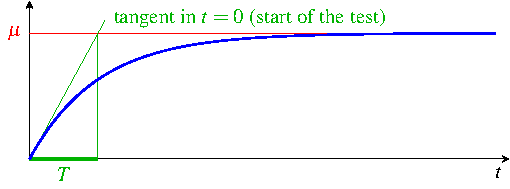
\includegraphics[width=0.55\columnwidth]{./Unit-06/img/FOstepResponse.pdf}
 \end{center}
 \begin{itemize}[<+-| alert@+>]
 \item \vspace{-4mm}When you know nothing about the system you need to control, but you know\\
       what is the input and what is the output, a viable way to get a model,\\
       is to perform a \TC{step test}.
 \item If the response resembles the first-order one above, you can read $\mu$\\
       and $T$ on the response record.
 \item Recall however that the $t$ axis is a CT one: seconds, minutes,...\\
       NOT samples, we still have to decide $T_s$ for our control.
 \end{itemize}
\end{frame}

\begin{frame}[label={pag:FOsystem-DT}]
\frametitleTC{Sampled-signal case}
\framesubtitleTC{Dominantly first-order asymptotically stable process}
\myPause
 \begin{itemize}[<+-| alert@+>]
 \item Now let us turn the system to DT as we already did:
       \begin{displaymath}
        \dot{y}(t) = -\frac{1}{T}y(t) + \frac{\mu}{T} u(t) \quad \Rightarrow \quad
        \frac{y(k)-y(k-1)}{T_s} = -\frac{1}{T}y(k) + \frac{\mu}{T} u(k). 
       \end{displaymath}
 \item This allows us to compute the DT transfer function as
       \begin{displaymath}
        \frac{1-z^{-1}{T_s}}y(k) = -\frac{1}{T}y(k) + \frac{\mu}{T} u(k) \; \Rightarrow \;
        P(z) = \frac{y(k)}{u(k)} = \frac{\mu\frac{T_s}{T+T_s}z}{z-\frac{T}{T+T_s}}.
       \end{displaymath}
 \item Quite expectedly, we have a first-order DT system whose parameters\\
       depend on $T_s$, i.e.,
       \begin{displaymath}
        P(z) = \frac{\rho z}{z-p}, \qquad
        \rho = \mu\frac{T_s}{T+T_s}, \quad
        p    = \frac{T}{T+T_s}.
       \end{displaymath}
 \end{itemize}
\end{frame}

\begin{frame}
\frametitleTC{Sampled-signal case}
\framesubtitleTC{Dominantly first-order asymptotically stable process}
\myPause
 \begin{itemize}[<+-| alert@+>]
 \item Results for different values of $T_s$ versus the CT case (dash-dot line):
       \begin{center}
        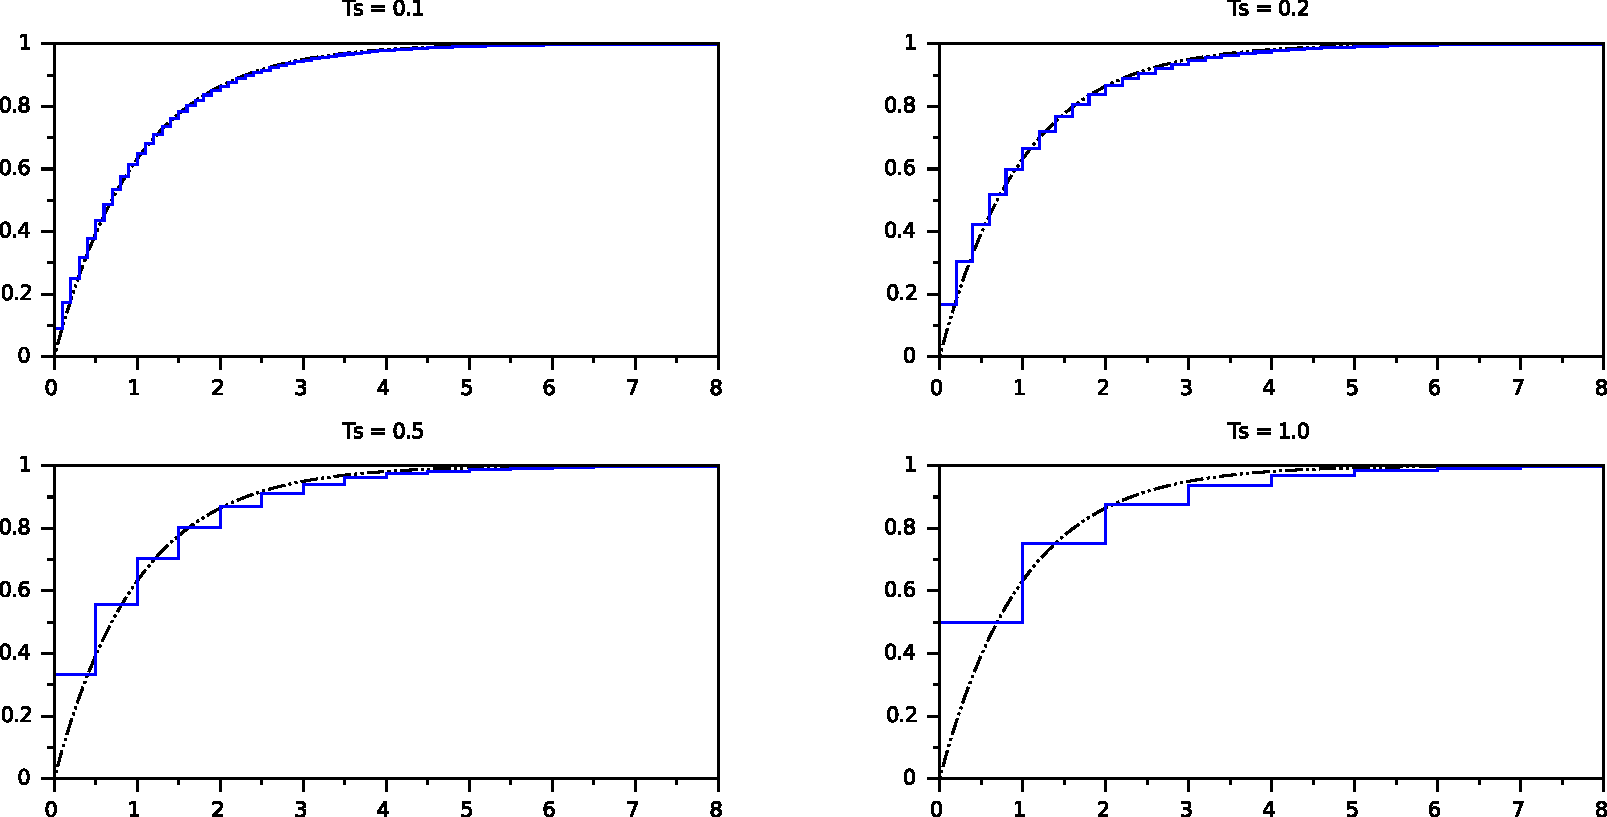
\includegraphics[width=0.60\columnwidth]{./Unit-06/img/CTvsDTexample-step.pdf}
       \end{center}
 \item \TC{Rule of thumb} to select $T_s$ for a representative DT approximation:\\
       at most 1/5 of $T$ (in our case $T=1$, $T_s=0.2$ is fine).
 \item Plenty of theory omitted, if interested ask for references...
 \end{itemize}
\end{frame}

\begin{frame}
\frametitleTC{A CT interpretation of the PI law}
\framesubtitleTC{useful for tuning}
\myPause
 \begin{itemize}[<+-| alert@+>]
 \item Can we interpret the PI control law
       \begin{displaymath}
        C_{PI}(z) = K \frac{z-\zeta}{z-1}
       \end{displaymath}
       in the continuous time, so as to derive $T_s$-independent parameters for it as well?
 \item Of course. To this end, let us split the P and the I action again.
 \item The P action has no dynamics, for it the DT and the CT domains\\
       are the same:
       \begin{displaymath}
        u_P(k) = K_P e(k), \quad
        u_P(t) = K_P e(t).
       \end{displaymath}
 \end{itemize}
\end{frame}

\begin{frame}
\frametitleTC{A CT interpretation of the PI law}
\framesubtitleTC{}
\myPause
 \begin{itemize}[<+-| alert@+>]
 \item The integral action in the CT domain is conversely a true integral:
       \begin{displaymath}
        u_I(t) = K_I \int_0^t e(\tau)d\tau.
       \end{displaymath}
 \item As an immediate consequence, then,
       \begin{displaymath}
        \dot{u}_I(t) = K_I e(t),
       \end{displaymath}
 \item and once again, we relate CT to DT by replacing the time derivative\\
       with the incremental ratio over one step of length $T_s$, which yields
       \begin{displaymath}
        \frac{u_I(k)-u_I(k-1)}{T_s}= K_I e(k).
       \end{displaymath}
 \end{itemize}
\end{frame}

\begin{frame}
\frametitleTC{A CT interpretation of the PI law}
\framesubtitleTC{}
\myPause
 \begin{itemize}[<+-| alert@+>]
 \item It is a convention of the PI(D) literature and practice to express $K_I$ as the\\
       proportional control gain divided by a time, which is dimensionally consistent,\\
       i.e., to write in the CT
       \begin{displaymath}
        u_P(t)       = K e(t), \quad
        \dot{u}_I(t) = \frac{K}{T_i} e(t)
       \end{displaymath}
       where $K$ is called (somehow improperly) the \TC{gain}, and $T_i$ the \TC{integral time}.
 \item This reflects in the DT controller
       \begin{displaymath}
        \begin{array}{rcl}
         u_P(k) &=& K e(k) \\
         u_I(k) &=& u_I(k-1) + \frac{KT_s}{T_i} e(k)
        \end{array}
       \end{displaymath}
 \item In transfer function form, then,
       {\small
       \begin{displaymath}
        C_{PI}(z) = \frac{u_P(k)+u_I(k)}{e(k)}
                  = K + \frac{zKT_s}{T_i(z-1)}
                  = \frac{K(T_i+T_s)}{T_i} \, \frac{z-\frac{T_i}{T_i+T_s}}{z-1}.
       \end{displaymath}
       }
 \end{itemize}
\end{frame}

\begin{frame}
\frametitleTC{A CT interpretation of PI and 1st order model}
\framesubtitleTC{again in a view to controller tuning}
\myPause
 \begin{itemize}[<+-| alert@+>]
 \item Let us look at the first-order process model and the PI controller, once their\\
       $T_s$-independent parameters -- $(\mu,T)$ for $P$, $(K,T_i)$ for $C$ -- are evidenced:
       \begin{displaymath}
        P(z)      = \mu \frac{\frac{T_s}{T+T_s} z}{z-\frac{T}{T+T_s}}, \qquad
        C_{PI}(z) = \frac{K(T_i+T_s)}{T_i} \, \frac{z-\frac{T_i}{T_i+T_s}}{z-1}.
       \end{displaymath}
 \item Since $T>0$ by hypothesis and so is obviously $T_s$ as well, the process pole\\
       is within the unit circle.
 \item We can therefore tune the PI by cancellation, but now to do this we\\
       set $T_i=T$, i.e., \TC{we operate in the CT domain}. Doing so produces 
       \begin{displaymath}
        L(z) = \mu \frac{\frac{T_s}{\ccancel[green]{T+T_s}} z}{\ccancel[red]{z-\frac{T}{T+T_s}}}
               \frac{K\ccancel[green]{(T+T_s)}}{T} \, \frac{\ccancel[red]{z-\frac{T}{T+T_s}}}{z-1}
             = \frac{\mu K T_s}{T} \frac{z}{z-1}.
       \end{displaymath}
 \end{itemize}
\end{frame}

\begin{frame}
\frametitleTC{A CT interpretation of control objectives}
\framesubtitleTC{}
\myPause
 \begin{center}
  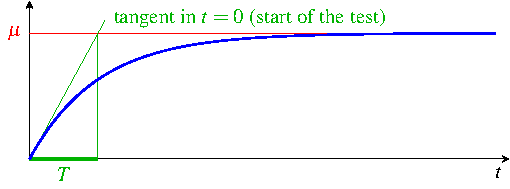
\includegraphics[width=0.45\columnwidth]{./Unit-06/img/FOstepResponse.pdf}
 \end{center}
 \begin{itemize}[<+-| alert@+>]
 \item If we want $y$ to reach $u$ within a certain time, the $y \rightarrow w$ continuous time system\\
       has to share the structure of the first-order process, but with $\mu=1$\\
       and a value of $T$ reflecting the desired speed.
 \item Since in the response above $y$ reaches its final value in about $5T$,\\
       if we want the closed-loop system to make $y$ reach $w$ and settle\\
       in a time $t_{set}$, then the required $T$ is $t_{set}/5$. Let us call this quantity\\
       $\lambda$ for brevity.
 \end{itemize}
\end{frame}

\begin{frame}[fragile]
\frametitleTC{Joining the pieces}
\framesubtitleTC{to the purpose of tuning}
\myPause
 \begin{itemize}[<+-| alert@+>]
 \item Substituting $\mu=1$ and $T=\lambda$ in the expression we found above for $P(z),$\\
       we get the objective $y/w$ transfer function as
       \begin{displaymath}
        G_{yw}^{\circ}(z) = \frac{\frac{T_s}{\lambda+T_s} z}{z-\frac{\lambda}{\lambda+T_s}}, \quad
        \lambda           = \frac{t_{set}}{5}
       \end{displaymath}
 \item We can then apply direct synthesis (wxMaxima):
       \begin{verbatim}
  P   : mu*Ts/(T+Ts)*z/(z-T/(T+Ts));
  Gywo: Ts/(lambda+Ts)*z/(z-lambda/(lambda+Ts));
  Csol: rhs(solve(P*C/(1+P*C)=Gywo,C)[1]);
       \end{verbatim}
 \end{itemize}
\end{frame}

\begin{frame}[fragile,label={pag:PItuning-lambda}]
\frametitleTC{Tuning}
\framesubtitleTC{direct synthesis for set point tracking -- CT setting}
\myPause
 \begin{itemize}[<+-| alert@+>]
 \item The result corresponds to the expression we already found for $C$, with
       \begin{displaymath}
        K   = \frac{T}{\lambda\mu}, \quad
        T_i = T.
       \end{displaymath}
 \item check (wxMaxima):
       {\small
       \begin{verbatim}
  K   : T/(mu*lambda);
  Ti  : T;
  Cchk: K*(Ti+Ts)/Ti*(z-Ti/(Ti+Ts))/(z-1); /* The C we got */
  ratsimp(Cchk-Csol);                      /* -> zero, OK  */
       \end{verbatim}
       }
 \item The ``direct synthesis for disturbance rejection'' case is left as a\\
       simple exercise (use wxMaxima). We now observe our result to\\
       make some important remarks.
 \end{itemize}
\end{frame}

\begin{frame}
\frametitleTC{Remarks}
\framesubtitleTC{direct synthesis for set point tracking -- CT setting}
\myPause
 \begin{itemize}[<+-| alert@+>]
 \item We showed that the idea of tuning by cancellation can be somehow applied\\
       in the CT domain as well.
 \item We have to say ``somehow'' because we do not possess the knowledge of\\
       \TC{CT transfer function}.
 \item Such an object can be defined, however, and the DT theory we saw can be\\
       completed with its CT counterpart.
 \item In fact, just to notice, the CT side of the matter was born far before.
 \end{itemize}
\end{frame}

\begin{frame}
\frametitleTC{Remarks}
\framesubtitleTC{general ideas to remember}
\myPause
 \begin{itemize}[<+-| alert@+>]
 \item You can derive a ``model for control'' that is VERY SIMPLE, yet enough\\
       for tuning, even just by looking at recorded data.
 \item So simple models are often flagged as ``too simple to provide realistic\\
       guarantees''...
 \item ...but basically by researchers who do not know about the Systems and Control\\
       Theory (no judgement, just mentioning facts).
 \item Be careful about ``realism'', and always consider the PURPOSE of\\
       your model.
 \item In the end, for example, temperature is molecular motion, but luckily\\
       we do not need to follow individual molecules to do temperature\\
       control \smiley.
 \end{itemize}
\end{frame}

\begin{frame}
\frametitleTC{Remarks}
\framesubtitleTC{General ideas to remember}
\myPause
 \begin{itemize}[<+-| alert@+>]
 \item On the symmetric front, be careful about the REPRESENTATIVENESS\\
       of your model.
 \item If you have knowledge of the phenomenon, that is a great advantage.
 \item If you need to rely on data, be sure to explore all the relevant dynamics.
 \item Experiment design is itself a discipline, explore it and/or get in touch with\\
       experts of the Identification Theory.
 \item And in general, be cautious about benchmarks that assert they are ``general''\\
       just because e.g. they contain a ``large'' number of ``heterogeneous''\\
       applications.
 \item By themselves, such statements provide NO guarantee that the\\
       tuned control will not have to face a totally unforeseen dynamics.
 \end{itemize}
\end{frame}

\begin{frame}
\frametitleTC{Remarks}
\framesubtitleTC{Even more general ideas to remember}
\myPause
 \begin{itemize}[<+-| alert@+>]
 \item To set up a control \TC{you need a model}.
 \item A model for that purpose is a \TC{dynamic system}.
 \item If you need formal guarantees on control, you need the Systems Theory.
 \item []{\small
       \begin{quote}
        There is no royal road to geometry.\\
        \vspace{1mm}\hspace{70mm}Euclid
       \end{quote}
       }
 \item However, never stretch a model beyond its purpose.
 \item []{\small
       \begin{quote}
        Since all models are wrong the scientist cannot obtain a ``correct'' one\\
        by excessive elaboration. On the contrary following William of Occam\\
        he should seek an economical description of natural phenomena.\\
        Just as the ability to devise simple but evocative models\\
        is the signature of the great scientist so overelaboration\\
        and overparameterization is often the mark of mediocrity.\\
        \vspace{1mm}\hspace{70mm}George Box
       \end{quote}
       }
 \item []...often summarised as ``all models are wrong, some are useful''. 
 \end{itemize}
\end{frame}
